\section{Environment}


\subsection{Microcontroller}
\frame
{
\frametitle{Arduino}

\begin{itemize}
\item Environment to program a micro-controller
	\begin{itemize}
	\item Board with full hardware
		\begin{itemize}
		\item USB - Serial
		\item Power supply
		\item Wide up pin distance
		\end{itemize}
	\item Software to program
	\item Wide up pin distance
	\end{itemize}
\end{itemize}
}


\frame
{
\frametitle{Arduino}
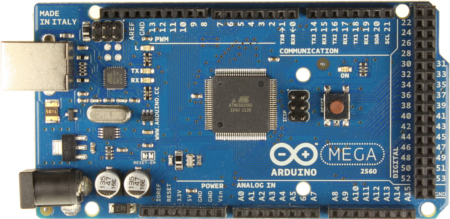
\includegraphics[width=\textwidth]{picturesArduino/arduinoMega2560_R3_Front.jpg}
}


\frame
{
\frametitle{Programming a microcontroller}

\begin{itemize}
\item Data types differs
	\begin{itemize}
	\item int (16)
	\item long (32)
	\item float (32)
	\item double (32)
	\end{itemize}
\item Floating-point numbers
	\begin{itemize}
	\item Very slow
	\item Precision 6-7 digits
	\end{itemize}
\item IO
	\begin{itemize}
	\item Binary I/O
	\item Analog, PWM
	\item UART / RS232
	\item I2C / TWI
	\end{itemize}
\end{itemize}
}


\frame
{
\frametitle{PWM - Analog Output}

\begin{itemize}
\item Principe
	\begin{itemize}
	\item Swith on and of
	\end{itemize}
\item Is needed for
	\begin{itemize}
	\item Analog Voltage (Smoothing Capacitors)
		\begin{itemize}
		\item Dim Leds, ... 
		\item Reference Voltage for Sensors
		\end{itemize}
	\item Control other devices
		\begin{itemize}
		\item Motor driver
		\item Servo
		\end{itemize}
	\end{itemize}
\end{itemize}
}


\frame
{
\frametitle{PWM - Analog Output}
\resizebox{\textwidth}{0.9\textheight}{
\tikzstyle{line}=[color=black,line width=1.5pt]
\newcommand*{\drawPWMschematic}[1]{
	\pgfmathsetmacro{\value}{#1 / 255}
	\pgfmathtruncatemacro{\dutyCycle}{round(100 * \value)}
	\draw(3,1) node[above]{\makebox[0pt][l]{\dutyCycle\%~Duty Cycle - analogWrite(#1)} };
	\draw(-0.5,1) node[left]{\makebox[0pt][l]{5V} };
	\draw(-0.5,0) node[left]{\makebox[0pt][l]{0V} };
	\pgfmathsetmacro{\offValue}{1 - \value}	
	\drawSquarewave{line}{5}{\value}{\offValue}{2}{1}
}
\makebox[\linewidth]{
\begin{tikzpicture}
	\newcounter{cpos}
	\foreach \n in {0,64,127,191,255} {
		\pgfmathsetmacro{\pos}{\value{cpos} * 1.65}
		\begin{scope}[shift={(0,\pos )}]
			\drawPWMschematic{\n}
		\end{scope}
		\stepcounter{cpos}
        }
\end{tikzpicture}
}
}
}


\frame
{
\frametitle{Programming a Microcontroller}

\begin{itemize}
\item Interrupts
	\begin{itemize}
	\item Timer
	\item Pin change
	\end{itemize}
\item Exception Result
	\begin{itemize}
	\item Continue
	\item Restart
	\end{itemize}
\item Watchdog
\end{itemize}
}
